\chapter{膜与膜运输}\label{ch:b1:membranes-transport}

把一个红\omterm{def:b1:cell-unit-of-life:cell}{细胞}放入纯水中，它会在一
秒钟内膨胀破裂；放入浓盐溶液中，它则会皱缩。把它放回\omterm{def:b1:mammal-organization:compartments}{血浆}中，
它能保持双凹圆盘形状长达四个月，其间每一秒都在将钠泵出、将钾泵入。完成这一切的膜
厚五纳米——是一层两个分子厚的脂质薄膜，
其中嵌有蛋白质——它是\omterm{def:b1:cell-unit-of-life:cell}{细胞}与外界之间的边界，
在\cref{ch:b1:organism-environment}中讨论的每一种交换，
最终都在这里完成。本章
阐述膜的结构、无需借助蛋白质即可穿膜的物质的物理过程、
承担其余运输任务的蛋白质（载体、泵和通道）、
这种运输产生的电位，以及
蛋白质无法运送之物所依赖的囊泡。

\section{流动镶嵌}

\begin{definition}[质膜]\label{def:b1:membranes-transport:membrane}
\emph{质膜}\index{质膜}——以及\omterm{def:b1:cell-unit-of-life:cell}{细胞}的每一层膜——
是一种\emph{脂双层}\index{脂双层}，
厚约\qty{5}{nm}，由两层磷脂组成：
（见\cref{ch:b1:lipids}），疏水尾部彼此相对，
极性头部朝向两侧的水相，尾部之间夹有胆固醇，并
有\emph{膜蛋白}\index{膜蛋白}嵌入其中或附着于其上。
在\emph{流动镶嵌}\index{流动镶嵌}模型（Singer 与 Nicolson, 1972）中，脂双层
是一种二维流体，其中脂质与蛋白质可侧向扩散，
而蛋白质是由彼此独立的单位组成的镶嵌，并非一层连续的外衣。
两个表面并不相同：与脂质和蛋白质相连的糖类
只朝向外侧（即\emph{糖萼}），而有些磷脂
仅局限于双层的其中一层。
\end{definition}

\begin{omfigure}
\begin{tikzpicture}[font=\footnotesize, line cap=round]
  % bilayer: heads as circles, tails as lines
  \foreach \i in {0,...,21} {
    \pgfmathsetmacro{\x}{0.42*\i}
    \fill[omDef!60] (\x,1.35) circle (0.16);
    \draw[omDef!70!black, thick] (\x-0.07,1.2) -- (\x-0.07,0.55) (\x+0.07,1.2) -- (\x+0.07,0.55);
    \fill[omDef!60] (\x,-0.35) circle (0.16);
    \draw[omDef!70!black, thick] (\x-0.07,-0.2) -- (\x-0.07,0.45) (\x+0.07,-0.2) -- (\x+0.07,0.45);
  }
  % cholesterol
  \foreach \x in {1.9,6.1,8.2} { \draw[omProp, very thick] (\x,1.1) -- (\x,0.6); \fill[omProp] (\x,1.15) circle (0.08); }
  % integral protein spanning (channel)
  \draw[thick, omThm!80!black, fill=omThm!30, rounded corners=3pt] (3.0,-0.7) rectangle (3.55,1.7);
  \draw[thick, omThm!80!black, fill=omThm!30, rounded corners=3pt] (3.85,-0.7) rectangle (4.4,1.7);
  \fill[white] (3.55,-0.6) rectangle (3.85,1.6);
  % integral protein (carrier)
  \draw[thick, omThm!80!black, fill=omThm!30, rounded corners=5pt] (6.8,-0.75) rectangle (7.7,1.75);
  % peripheral protein
  \draw[thick, omExo!80!black, fill=omExo!30] (5.3,1.75) ellipse (0.5 and 0.28);
  % glycocalyx sugar chains on outer face
  \foreach \x in {0.5,1.3,2.5,4.15,7.25,8.4} { \draw[omProp!80!black, thick] (\x,1.5) .. controls (\x+0.15,1.85) and (\x-0.15,2.1) .. (\x+0.1,2.4); \fill[omProp!70] (\x+0.1,2.45) circle (0.07); }
  % labels
  \node[anchor=east] at (-0.3,1.35) {极性头部};
  \node[anchor=east] at (-0.3,0.5) {疏水尾部};
  \node[anchor=east] at (-0.3,-0.35) {极性头部};
  \node[anchor=west, align=left] at (9.2,2.2) {糖链：仅在外侧};
  \node[anchor=west, align=left] at (9.2,0.5) {\qty{5}{nm}};
  \node[anchor=north] at (3.7,-0.95) {通道蛋白};
  \node[anchor=north] at (7.25,-0.95) {载体蛋白};
  \node[anchor=south] at (5.3,2.6) {外周蛋白};
  \node[anchor=north, omProp] at (1.5,-1.0) {胆固醇};
  \node[anchor=south east, gray] at (-0.3,2.4) {外侧};
  \node[anchor=north east, gray] at (-0.3,-0.95) {细胞溶胶};
  \draw[<->, gray] (9.05,1.35+0.16) -- (9.05,-0.35-0.16);
\end{tikzpicture}

{\small \omterm{def:b1:membranes-transport:membrane}{流动镶嵌}。两层磷脂，尾部朝内，
胆固醇位于其间；\omterm{def:b1:membranes-transport:proteins}{整合蛋白}贯穿
双层（一种为带孔道的\omterm{def:b1:membranes-transport:transporters}{通道蛋白}，另一种为\omterm{def:b1:membranes-transport:transporters}{载体蛋白}），一个外周蛋白附着于
其中一侧表面，糖链仅位于外侧表面。}
\end{omfigure}

\begin{omfigure}
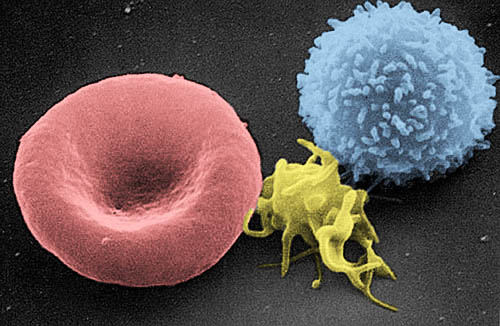
\includegraphics[width=0.4\linewidth]{images/book3/red-cells-nci.jpg}

{\small 扫描\omterm{prop:b1:cell-unit-of-life:microscopes}{电子显微镜}下的一个红\omterm{def:b1:cell-unit-of-life:cell}{细胞}、一个血小板和一个淋巴\omterm{def:b1:cell-unit-of-life:cell}{细胞}
（已着色）。红\omterm{def:b1:cell-unit-of-life:cell}{细胞}的双凹形状由膜下的蛋白质网维持，
它能经受住比自身更窄的毛细血管的挤压，
并存活四个月。图片：
美国国家癌症研究所，公有领域。}
\end{omfigure}

\begin{proposition}[膜是双层且具流动性]\label{prop:b1:membranes-transport:evidence}
\omterm{def:b1:membranes-transport:membrane}{质膜}恰为两个脂质分子厚，且其组分
可在膜平面内运动。
\end{proposition}
\begin{proof}[证据]
Gorter 与 Grendel（1925）从已知数目的
红\omterm{def:b1:cell-unit-of-life:cell}{细胞}中提取脂质，将其铺展于水面形成单分子层，其面积
恰为\omterm{def:b1:cell-unit-of-life:cell}{细胞}总表面积的两倍，因此膜是双层结构。
\omterm{prop:b1:cell-unit-of-life:microscopes}{电子显微镜}下，每一层膜都呈现为两条暗线
（染色的头部）包围着一条浅色的核心（尾部），总厚\qty{5}{nm}。
Frye 与 Edidin（1970）将一个小鼠\omterm{def:b1:cell-unit-of-life:cell}{细胞}与一个人\omterm{def:b1:cell-unit-of-life:cell}{细胞}融合，后者的
表面蛋白已用两种颜色的染料标记；
在\qty{37}{\celsius}下经过四十分钟，两种颜色在杂交\omterm{def:b1:cell-unit-of-life:cell}{细胞}上
已完全混合；而在\qty{4}{\celsius}下则不然，那时
脂质几乎呈固态。用激光漂白荧光\omterm{def:b1:membranes-transport:membrane}{膜蛋白}上的一个斑点，
并观察荧光随未漂白分子扩散进入而恢复，
这一方法（FRAP）测量侧向扩散：
在 $\qty{1}{\micro m^2}$ 的面积内，脂质数秒即可恢复，蛋白质较慢，
与\omterm{def:b1:eukaryotic-cell:cytoskeleton}{细胞骨架}锚定的蛋白质则为零。
\end{proof}

\begin{definition}[膜蛋白]\label{def:b1:membranes-transport:proteins}
\emph{整合蛋白}\index{整合蛋白}横跨
双层，含一个或多个疏水螺旋，只能用去污剂提取；
\emph{外周}蛋白则结合于膜的一侧表面。按功能分，
\emph{转运蛋白}（\omterm{def:b1:membranes-transport:transporters}{通道蛋白}、\omterm{def:b1:membranes-transport:transporters}{载体蛋白}和泵）、
\emph{受体}在膜外结合信号，在膜内发挥作用，
\emph{酶}、\emph{锚定蛋白}，将\omterm{def:b1:eukaryotic-cell:cytoskeleton}{细胞骨架}连接到
\omterm{def:b1:body-plans-tissues:connective}{细胞外基质}上，以及\emph{识别}蛋白，其携带的糖类
可供\omterm{def:b1:cell-unit-of-life:cell}{细胞}彼此辨认。蛋白质约占典型膜质量的一半，
却承担了膜的几乎全部功能。
\end{definition}

\section{不借助蛋白质的跨膜运输}

\begin{proposition}[双层的通透性]\label{prop:b1:membranes-transport:permeability}
\index{通透性}
纯\omterm{def:b1:membranes-transport:membrane}{脂双层}可自由通透小的非极性分子
（$\mathrm{O_2}$、$\mathrm{CO_2}$、$\mathrm{N_2}$、类固醇），较易通透
小的不带电极性分子（水、尿素、乙醇），
难以通透较大的极性分子（葡萄糖、氨基酸），并且
实际上不能通透离子（$\mathrm{Na^+}$、$\mathrm{K^+}$、
$\mathrm{Cl^-}$、$\mathrm{H^+}$）以及大分子。
通透性跨越十二个数量级，
从水的 $\qty{e-2}{cm/s}$ 到 $\qty{e-14}{cm/s}$（$\mathrm{Na^+}$）：
疏水核心厚 \qty{3}{nm}，能让溶于
油的物质通过，带电荷的则被阻挡。
\end{proposition}

\begin{theorem}[扩散的菲克定律]\label{thm:b1:membranes-transport:fick}
\index{菲克定律}\index{扩散}
溶质的净通量 $J$ 穿过面积为 $S$ 的膜（摩尔
每秒）与膜两侧的浓度差成正比：
\[
J = P\,S\,(c_{\text{外}} - c_{\text{内}}),
\]
其中\emph{通透系数} $P$（以 \unit{m/s} 计）综合
了溶质在膜中的扩散系数、其在脂质中的
溶解度与膜的厚度（$P = DK/\ell$）。
扩散不需要能量，总是顺梯度进行，属于
\emph{被动运输}\index{被动运输}。
\end{theorem}
\begin{proof}
溶质在膜内沿线性浓度分布
由 $Kc_{\text{外}}$ 降至 $Kc_{\text{内}}$（$K$ 为脂质与水之间的
分配系数）；体相中的菲克第一定律
在体相中 $J/S = -D\,\dd c/\dd x$，由此得 $J/S = DK(c_{\text{外}} -
c_{\text{内}})/\ell$。
\end{proof}

\begin{definition}[渗透作用，水势]\label{def:b1:membranes-transport:osmosis}
\emph{渗透作用}\index{渗透作用}是水穿过只允许水通过、不允许溶质通过的膜的净扩散，
方向由水浓度较高（溶质较少）的溶液一侧
指向水浓度较低的一侧。
常用\emph{水
势}\index{水势} $\Psi$，即以压强表示的水的化学势，
规定纯水在大气压强下的值
为零：
\[
\Psi = \Psi_s + \Psi_p, \qquad \Psi_s = -RTc_s ,
\]
其中 $\Psi_s$ 即\emph{溶质势}\index{溶质势}，它随溶质总浓度 $c_s$ 增大而降低
（以渗透摩尔每升计，范托夫定律），而 $\Psi_p$ 为
\emph{压力
势}\index{压力势}，是高出大气压的静水压；
水由 $\Psi$ 较高处流向较低处。在
\qty{25}{\celsius} 时，$RT = \qty{2.48}{MPa.L/mol}$。一
\qty{0.3}{osmol/L} 的溶液，其 $\Psi_s = \qty{-0.74}{MPa}$。
溶液对\omterm{def:b1:cell-unit-of-life:cell}{细胞}而言，无净水流动时为\emph{等渗}\index{等渗}，
有水进入时为\emph{低渗}，有水流出时为\emph{高渗}。
\end{definition}

\begin{omfigure}
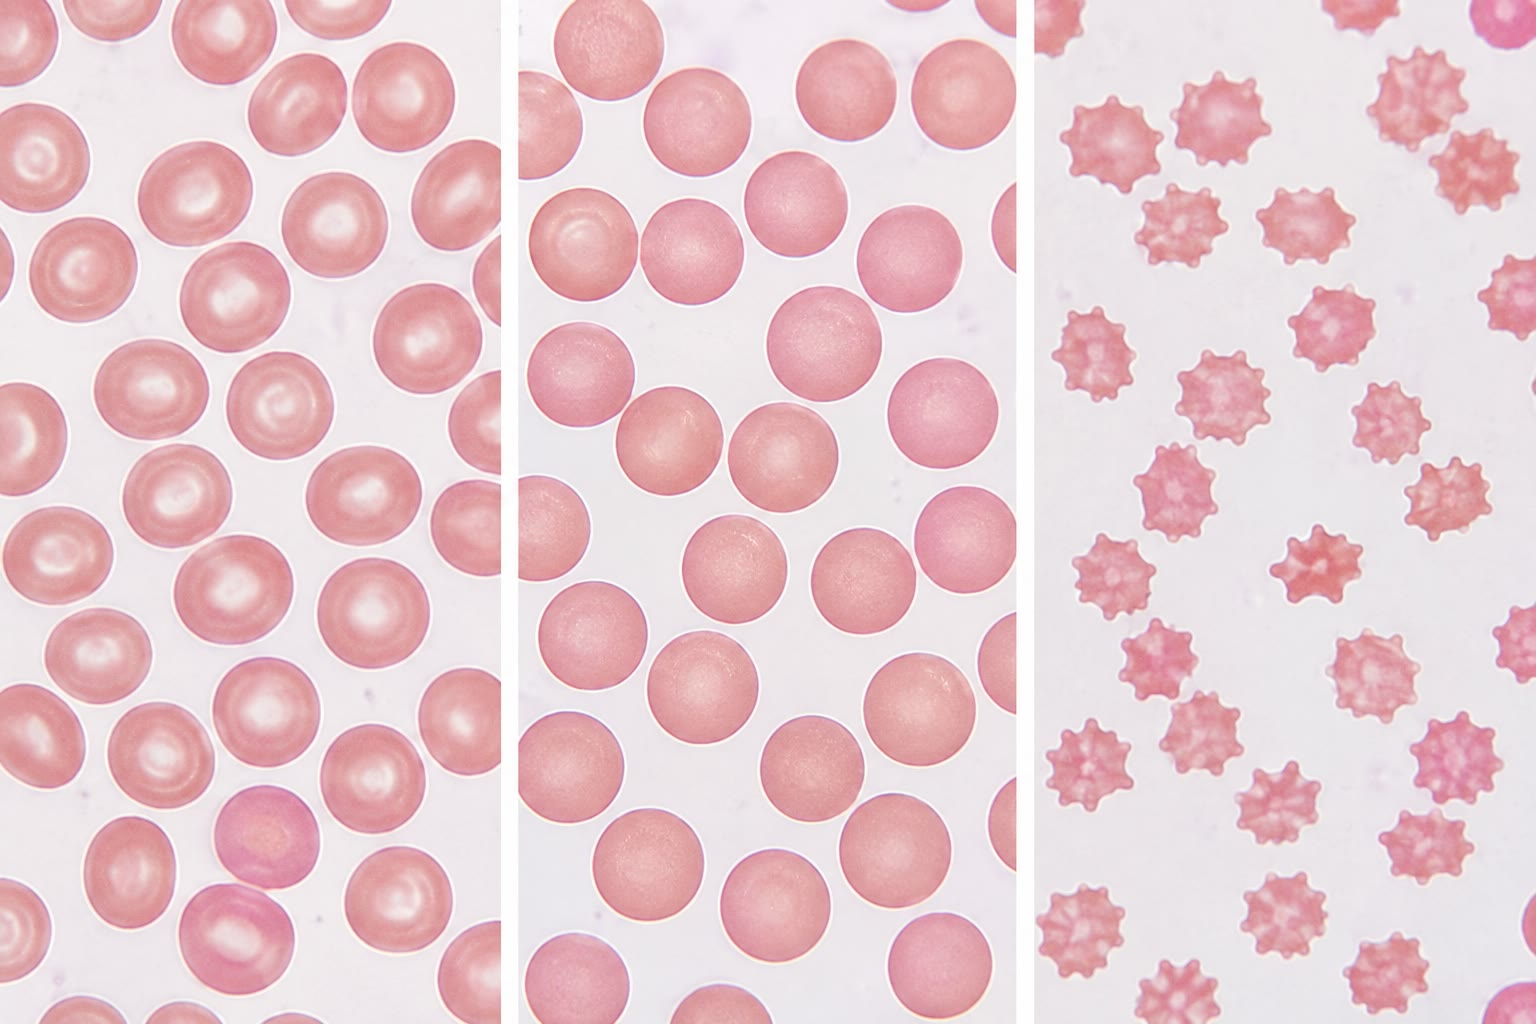
\includegraphics[width=0.78\linewidth]{images/book3/ai/b3-07-red-cells-osmosis.jpg}

{\small 红\omterm{def:b1:cell-unit-of-life:cell}{细胞}在\omterm{def:b1:membranes-transport:osmosis}{等渗}溶液中（双凹圆盘状）、在
低渗溶液中（膨胀成球形，即将破裂）以及在
高渗溶液中（皱缩并呈棘状）。水的流动由\omterm{def:b1:membranes-transport:osmosis}{水势}决定；
\omterm{def:b1:cell-unit-of-life:cell}{细胞}没有\omterm{def:b1:eukaryotic-cell:plantcell}{细胞壁}来抵抗。}
\end{omfigure}

\begin{omfigure}
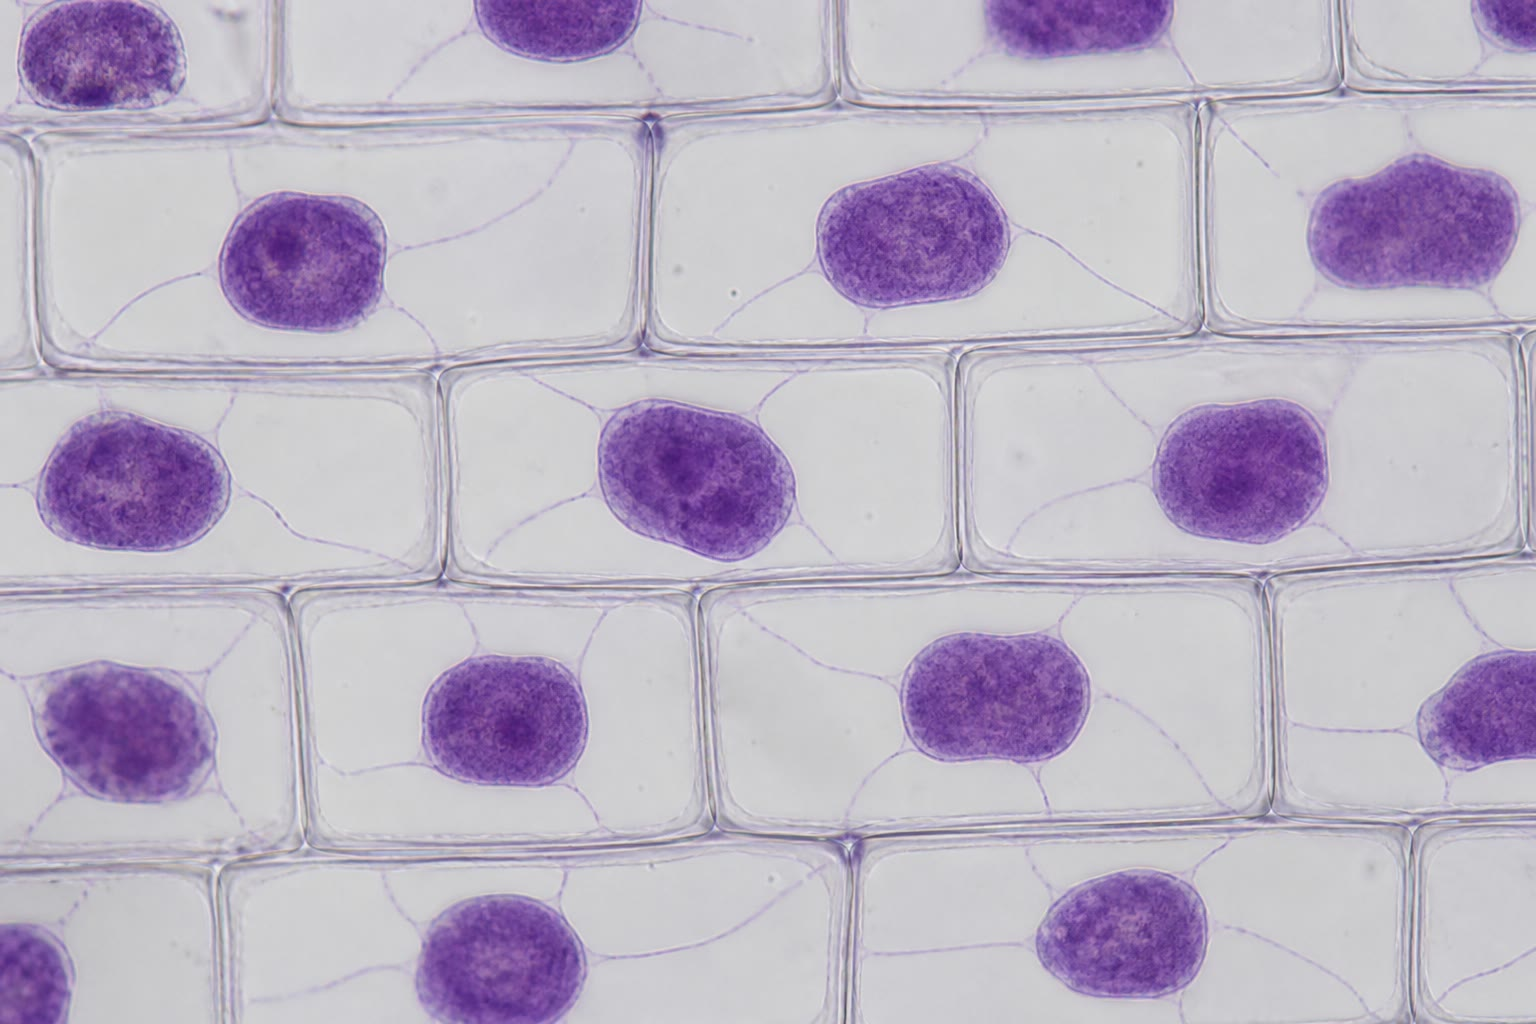
\includegraphics[width=0.6\linewidth]{images/book3/ai/b3-07-plasmolysis.jpg}

{\small 质壁分离：洋葱\omterm{def:b1:flowering-plant-organization:tissues}{表皮}置于强盐溶液中。
每个\omterm{def:b1:cell-unit-of-life:cell}{细胞}的原生\omterm{def:b1:eukaryotic-cell:plastid}{质体}已失水，与坚硬的
\omterm{def:b1:eukaryotic-cell:plantcell}{细胞壁}分离，\omterm{def:b1:eukaryotic-cell:plantcell}{细胞壁}使\omterm{def:b1:cell-unit-of-life:cell}{细胞}保持形状。在水中，原生\omterm{def:b1:eukaryotic-cell:plastid}{质体}会
重新膨胀，紧贴\omterm{def:b1:eukaryotic-cell:plantcell}{细胞壁}并停止，\omterm{def:b1:cell-unit-of-life:cell}{细胞}呈充盈状态。}
\end{omfigure}

\begin{example}[红细胞置于三种溶液中]\label{ex:b1:membranes-transport:redcell}
\omterm{def:b1:mammal-organization:compartments}{血浆}为 \qty{0.3}{osmol/L}：两侧 $\Psi_s = \qty{-0.74}{MPa}$，
无净流动。在纯水（$\Psi = 0$）中，\omterm{def:b1:cell-unit-of-life:cell}{细胞}内
为 \qty{-0.74}{MPa}，\omterm{def:b1:cell-unit-of-life:cell}{细胞}吸水直至其膜（只能伸展几个百分点）
破裂。在 \qty{0.6}{osmol/L} 盐溶液中，\omterm{def:b1:cell-unit-of-life:cell}{细胞}失水，
直至内部浓度相同，体积减为一半。植物
\omterm{def:b1:cell-unit-of-life:cell}{细胞}在纯水中不会破裂：水进入时，\omterm{def:b1:eukaryotic-cell:plantcell}{细胞壁}被拉伸，
$\Psi_p$ 升高直至 $\Psi_p = -\Psi_s$，\omterm{def:b1:cell-unit-of-life:cell}{细胞}内\omterm{def:b1:membranes-transport:osmosis}{水势}为零，
水流停止，\omterm{def:b1:cell-unit-of-life:cell}{细胞}呈充盈状态，\omterm{def:b1:eukaryotic-cell:plantcell}{膨压}为
\qty{0.74}{MPa}。
\end{example}

\begin{method}[水势计算]\label{met:b1:membranes-transport:psi}
\begin{enumerate}
  \item 将每种溶质浓度换算为渗透摩尔（解离成两个离子的盐计两次），
        并计算 $\Psi_s =
        -RTc_s$。
  \item 加上压力项：在开口容器中的溶液或动物\omterm{def:b1:cell-unit-of-life:cell}{细胞}内，$\Psi_p = 0$，
        充盈植物\omterm{def:b1:cell-unit-of-life:cell}{细胞}为正，
        \omterm{def:b1:flowering-plant-organization:tissues}{木质部}\omterm{def:b1:flowering-plant-organization:tissues}{导管}中处于张力下的水为负。
  \item 水流向较低的 $\Psi$。两个 $\Psi$ 相等时即达到平衡，
        动物\omterm{def:b1:cell-unit-of-life:cell}{细胞}借稀释内容物达到，
        植物\omterm{def:b1:cell-unit-of-life:cell}{细胞}则借压强升高达到。
  \item 以结果的正负号表示流动方向，其
        大小表示驱动力；流速还取决于
        膜的水通透性，而该通透性
        经\omterm{def:b1:membranes-transport:transporters}{水通道蛋白}提高了一百倍。
\end{enumerate}
\end{method}

\section{转运蛋白}

\begin{definition}[通道蛋白、载体蛋白和泵]\label{def:b1:membranes-transport:transporters}
\emph{通道蛋白}\index{通道蛋白}是\omterm{def:b1:membranes-transport:proteins}{整合蛋白}，内有
充水的孔道，特定离子或小分子可借此
沿梯度扩散，速率最高可达 $10^8$ 每秒；许多
是\emph{门控}的，会因电压、配体或
机械力而开放。\emph{水通道蛋白}\index{水通道蛋白}
即运输水的通道。\emph{载体蛋白}\index{载体蛋白}在一侧面结合溶质，
改变构象，并在另一侧释放，每秒至多
一千次；红\omterm{def:b1:cell-unit-of-life:cell}{细胞}的葡萄糖转运蛋白即为其一。
顺梯度运作的通道蛋白与载体蛋白进行\emph{协助
扩散}\index{协助扩散}，属\omterm{thm:b1:membranes-transport:fick}{被动运输}，但具选择性且
可饱和。\emph{泵}\index{泵}是偶联溶质逆梯度转运
与 ATP 水解的载体，属于
\emph{原发性主动运输}\index{主动运输}。
\emph{钠钾泵}\index{钠钾泵}见于动物
\omterm{def:b1:cell-unit-of-life:cell}{细胞}，每消耗一分子 ATP 向外排出三个 $\mathrm{Na^+}$，向内输入两个
$\mathrm{K^+}$；植物、真菌和细菌膜上的\emph{质子泵}
向外排出 $\mathrm{H^+}$。
\end{definition}

\begin{omfigure}
\begin{tikzpicture}[font=\footnotesize, >=Stealth, line cap=round]
  % membrane band
  \fill[omDef!15] (0,0) rectangle (13.1,1.2);
  \draw[omDef!60!black] (0,0) -- (13.1,0) (0,1.2) -- (13.1,1.2);
  \node[anchor=east, gray, align=right] at (-0.15,1.5) {外侧 \\ （高 $\mathrm{Na^+}$，低 $\mathrm{K^+}$）};
  \node[anchor=east, gray, align=right] at (-0.15,-0.3) {细胞溶胶 \\ （低 $\mathrm{Na^+}$，高 $\mathrm{K^+}$）};
  % simple diffusion
  \draw[->, thick, omProp] (1.0,2.0) -- (1.0,-0.8);
  \node[anchor=south, align=center] at (1.0,2.1) {简单扩散 \\ $\mathrm{O_2}$、$\mathrm{CO_2}$};
  % channel
  \draw[thick, omThm!80!black, fill=omThm!30, rounded corners=2pt] (2.6,-0.2) rectangle (3.0,1.4);
  \draw[thick, omThm!80!black, fill=omThm!30, rounded corners=2pt] (3.3,-0.2) rectangle (3.7,1.4);
  \draw[->, thick, omProp] (3.15,2.0) -- (3.15,-0.8);
  \node[anchor=south, align=center] at (3.15,2.1) {通道蛋白 \\ $\mathrm{K^+}$、水};
  % carrier (facilitated)
  \draw[thick, omThm!80!black, fill=omThm!30, rounded corners=5pt] (5.0,-0.3) rectangle (6.0,1.5);
  \draw[->, thick, omProp] (5.5,2.0) -- (5.5,1.55);
  \draw[->, thick, omProp] (5.5,-0.35) -- (5.5,-0.8);
  \node[anchor=south, align=center] at (5.5,2.1) {载体蛋白 \\ 葡萄糖};
  \node[align=center, font=\scriptsize] at (5.5,0.6) {结合，\\ 翻转};
  % pump
  \draw[thick, omExo!80!black, fill=omExo!30, rounded corners=5pt] (7.5,-0.3) rectangle (8.7,1.5);
  \draw[->, very thick, omExo!80!black] (7.8,-0.8) -- (7.8,2.0);
  \draw[->, very thick, omExo!80!black] (8.4,2.0) -- (8.4,-0.8);
  \node[anchor=south, align=center] at (8.1,2.1) {泵 \\ 排出 $3\,\mathrm{Na^+}$，输入 $2\,\mathrm{K^+}$};
  \node[anchor=north, align=center, font=\scriptsize] at (8.1,-0.85) {ATP $\to$ ADP};
  % secondary active (symport)
  \draw[thick, omThm!80!black, fill=omThm!30, rounded corners=5pt] (11.0,-0.3) rectangle (12.2,1.5);
  \draw[->, very thick, omProp] (11.3,2.0) -- (11.3,-0.8);
  \draw[->, very thick, omExo!80!black] (11.9,2.0) -- (11.9,-0.8);
  \node[anchor=south, align=center] at (11.6,2.1) {同向转运体 \\ $\mathrm{Na^+}$ 下行，葡萄糖上行};
  \node[anchor=north, align=center, font=\scriptsize] at (11.6,-0.85) {继发性主动运输};
  \node[anchor=north west, align=left, gray, font=\scriptsize] at (0,-1.5) {橙色箭头：顺梯度（被动运输）；绿色：逆梯度（主动运输）};
\end{tikzpicture}

{\small 跨膜的五条途径：简单扩散穿过脂质；通道与
载体（\omterm{def:b1:membranes-transport:transporters}{协助扩散}，顺梯度）；\omterm{def:b1:membranes-transport:transporters}{钠钾泵}
（\omterm{def:b1:membranes-transport:transporters}{原发性主动运输}，消耗 ATP）；一种\omterm{prop:b1:membranes-transport:secondary}{同向转运体}，
利用泵建立的钠梯度，将葡萄糖逆梯度拖入\omterm{def:b1:cell-unit-of-life:cell}{细胞}，
属继发性\omterm{def:b1:membranes-transport:transporters}{主动运输}。}
\end{omfigure}

\begin{proposition}[继发性主动运输]\label{prop:b1:membranes-transport:secondary}
\index{继发性主动运输}
泵所建立的梯度是一种能量储备，供其他载体
消耗：\emph{同向转运体}\index{同向转运体}通过
将溶质与同向顺梯度运动的离子偶联，使其逆梯度上行（
如肠与肾中的钠–葡萄糖转运体、\omterm{def:b1:flowering-plant-organization:tissues}{韧皮部}中的
质子–蔗糖转运体）；
\emph{反向转运体}\index{反向转运体}则将溶质与
反向运动的离子偶联（如钠–钙交换体）。在动物\omterm{def:b1:cell-unit-of-life:cell}{细胞}中，
其能量来源是 $\mathrm{Na^+}$ 梯度；在植物、真菌和细菌中，
则是 $\mathrm{H^+}$ 梯度。
\end{proposition}

\begin{example}[动力学揭示机制]\label{ex:b1:membranes-transport:kinetics}
葡萄糖进入红\omterm{def:b1:cell-unit-of-life:cell}{细胞}的通量随外部
浓度升高而增加，随后在一最大值处趋于平缓，类似于酶
（\cref{ch:b1:enzymes}）：一种载体，可饱和，其 $K_m$ 约为
\qty{1.5}{mmol/L}；另一种相似的糖——甘露糖——与之竞争。尿素的通量
随其浓度成正比增加，不设上限：简单扩散。
葡萄糖进入肠\omterm{def:b1:cell-unit-of-life:cell}{细胞}的通量在肠腔中的钠被移除时
即告停止，或泵被哇巴因抑制时亦然，
此为继发性\omterm{def:b1:membranes-transport:transporters}{主动运输}。
\end{example}

\section{膜电位}

\begin{definition}[膜电位]\label{def:b1:membranes-transport:potential}
每个活\omterm{def:b1:cell-unit-of-life:cell}{细胞}的\omterm{def:b1:membranes-transport:membrane}{质膜}两侧都存在电势差，
即\emph{膜电位}\index{膜电位} $V_m = V_{\text{内}} - V_{\text{外}}$，内侧为负：
\omterm{def:b1:body-plans-tissues:nervous}{神经元}中为 \qty{-70}{mV}，肌纤维中为 \qty{-90}{mV}，
植物\omterm{def:b1:cell-unit-of-life:cell}{细胞}中则为 \qty{-120}{mV} 甚至更负。其成因在于膜
对两侧浓度不同的离子具有选择性通透性。
\end{definition}

\begin{theorem}[能斯特方程]\label{thm:b1:membranes-transport:nernst}
\index{能斯特方程}\index{平衡电位}
电荷数为 $z$ 的离子，其在膜两侧的浓度分别为 $c_{\text{外}}$ 与
$c_{\text{内}}$ 时该离子处于跨膜平衡——无净通量，
尽管膜对其可通透——当电位等于
其\emph{\omterm{thm:b1:membranes-transport:nernst}{平衡电位}}时，
\[
E_{\text{离子}} = \frac{RT}{zF}\,\ln\frac{c_{\text{外}}}{c_{\text{内}}}
= \frac{\qty{61.5}{mV}}{z}\,\log_{10}\frac{c_{\text{外}}}{c_{\text{内}}}
\quad (\qty{37}{\celsius}).
\]
对于 $\mathrm{K^+}$，外侧为 \qty{5}{mmol/L}，
内侧为 \qty{140}{mmol/L}，则 $E_K = 61.5\log(5/140) = \qty{-89}{mV}$；对于 $\mathrm{Na^+}$，
外侧为 \qty{145}{}，内侧为 \qty{12}{}，则 $E_{Na} = \qty{+67}{mV}$。
\end{theorem}
\begin{proof}
将一摩尔该离子由外侧移至内侧，自由能的变化
等于一项浓度项与一项电项之和：
\[
\Delta G = RT\ln\frac{c_{\text{内}}}{c_{\text{外}}} + zFV_m .
\]
平衡时 $\Delta G = 0$，由此得 $V_m = (RT/zF)\ln(c_{\text{外}}/c_{\text{内}})$。
改用以 10 为底的对数，并代入 $R = \qty{8.314}{J.mol^{-1}.K^{-1}}$，
$T = \qty{310}{K}$，$F = \qty{96485}{C/mol}$，即得数值形式。
\end{proof}

\begin{proposition}[静息电位的来源]\label{prop:b1:membranes-transport:resting}
静息膜对 $\mathrm{K^+}$（经开放的钾通道）的通透性远高于
对 $\mathrm{Na^+}$；$\mathrm{K^+}$ 沿浓度梯度外漏，
使内侧呈负，直至电性回拉与渗漏
近乎抵消。因此静息电位接近 $E_K$，并
因少量钠渗漏略向 $E_{Na}$ 偏移（戈德曼方程
按各离子的通透性对其能斯特项加权）。泵维持
渗漏原本会耗散的梯度；它还直接贡献
数毫伏的电位，因其每次排出三个电荷、
仅输入两个。
\end{proposition}
\begin{proof}[证据]
在鱿鱼轴突中，静息电位跟随 $E_K$，当外侧
钾浓度在较宽范围内变化时（高浓度下为斜率
每十倍 \qty{58}{mV} 的直线），并在低浓度时偏离之，
恰如小钠通透性所预示的那样。
以哇巴因阻断泵后，电位在数分钟内几乎不变，
随后随梯度耗尽而在数小时内衰减：
该电位是一种扩散电位，而泵是其
长期支持。
\end{proof}

\begin{omfigure}
\begin{tikzpicture}
\begin{semilogxaxis}[
  width=0.86\linewidth, height=6.2cm,
  axis x line=bottom, axis y line=left,
  xmin=0.8, xmax=200, ymin=-135, ymax=10,
  xlabel={外侧 $\mathrm{K^+}$ (\unit{mmol/L})}, ylabel={膜电位 (\unit{mV})},
  xlabel style={font=\small, at={(axis description cs:0.5,-0.12)}, anchor=north},
  ylabel style={font=\small},
  tick label style={font=\small}, xtick={1,10,100}, log ticks with fixed point, ytick={-120,-100,-80,-60,-40,-20,0},
  legend style={font=\small, at={(0.03,0.97)}, anchor=north west, draw=none},
  clip=false,
]
\addplot[thick, dashed, omDef, domain=0.8:200, samples=40] {58*log10(x/140)};
\addlegendentry{能斯特 $E_K$（斜率为每十倍 \qty{58}{mV}）}
\addplot[very thick, omThm, domain=0.8:200, samples=60] {58*log10((x+0.01*145)/(140+0.01*12))};
\addlegendentry{实测：$\mathrm{K^+}$ 加上少量 $\mathrm{Na^+}$ 漏流}
\draw[dashed, gray] (axis cs:5,-135) -- (axis cs:5,-82);
\node[font=\scriptsize, anchor=west] at (axis cs:5.5,-120) {生理浓度 \qty{5}{mmol/L}};
\end{semilogxaxis}
\end{tikzpicture}

{\small 静息电位随外侧钾浓度的变化。高钾浓度下，膜的行为类似钾电极，
并沿能斯特直线变化；低钾浓度下，
微弱的钠漏流把电位拉到
高于 $E_K$。}
\end{omfigure}

\begin{example}[泵的能量去向]\label{ex:b1:membranes-transport:pumpcost}
将一个 $\mathrm{Na^+}$ 泵出\omterm{def:b1:cell-unit-of-life:cell}{细胞}，克服从 \qty{12}{} 到 \qty{145}{mmol/L} 的浓度梯度
以及 \qty{-70}{mV} 的\omterm{def:b1:membranes-transport:potential}{膜电位}，耗能为 $RT\ln(145/12) + F\times 0.070 = 6.4 + 6.8 =
\qty{13.2}{kJ/mol}$；三个合计 \qty{40}{kJ}，另加两个
$\mathrm{K^+}$ 泵入\omterm{def:b1:cell-unit-of-life:cell}{细胞}，每个耗能 $RT\ln(140/5) - F\times 0.070 = 8.6 - 6.8 =
\qty{1.8}{kJ/mol}$ 每个，每循环共 \qty{43}{kJ}，对照
\omterm{def:b1:cell-unit-of-life:cell}{细胞}条件下一个 ATP 的 \qty{50}{kJ}。该泵接近其热力学极限运行，
并消耗静息动物约三分之一的
ATP，在脑中则占三分之二。
\end{example}

\section{大量运输}

\begin{proposition}[膜泡运输]\label{prop:b1:membranes-transport:vesicles}
大分子和颗粒穿过\omterm{def:b1:membranes-transport:membrane}{质膜}时，不经过
膜本身：通过\emph{胞吐作用}，囊泡与膜融合并将内容物
排向外侧；通过\emph{\omterm{def:b1:eukaryotic-cell:endocytosis}{胞吞作用}}，膜将物质包裹
入囊泡中（见\cref{ch:b1:eukaryotic-cell}）。两者都需要 ATP，两者都
既搬运膜，也搬运内容物，并且都保持膜的
方向性。穿过膜的三条途径——经由脂质、经由蛋白质、经由囊泡内部——
在三个方面具有选择性：按
溶解性、按分子识别、按被摄入物质的
选择。
\end{proposition}

\begin{example}[胆固醇的运送]\label{ex:b1:membranes-transport:ldl}
胆固醇在血液中装在包被有蛋白质的颗粒里运输，这些颗粒
对任何载体而言都太大。需要胆固醇的\omterm{def:b1:cell-unit-of-life:cell}{细胞}会表达
与颗粒结合的受体；颗粒与受体聚集于有被小窝，该小窝
内陷脱离，囊泡将颗粒送至\omterm{def:b1:eukaryotic-cell:endomembrane}{溶酶体}，
胆固醇在\omterm{def:b1:eukaryotic-cell:endomembrane}{溶酶体}中释放出来。若某人的受体有缺陷，
便无法清除这些颗粒：血液中的胆固醇加倍，动脉
成年早期即被堵塞。一种\omterm{def:b1:membranes-transport:membrane}{膜蛋白}，一种疾病。
\end{example}

\section{练习}

\begin{exercise}[$\star$]\label{exo:b1:membranes-transport:1}
用四句话描述\omterm{def:b1:membranes-transport:membrane}{流动镶嵌}模型：脂质、
蛋白质、流动性与不对称性。
\end{exercise}

\begin{exercise}[$\star$]\label{exo:b1:membranes-transport:2}
将 $\mathrm{O_2}$、葡萄糖、$\mathrm{Na^+}$、水和乙醇按
通过纯\omterm{def:b1:membranes-transport:membrane}{脂双层}的通透性排序，并说明理由。
\end{exercise}

\begin{exercise}[$\star$]\label{exo:b1:membranes-transport:3}
计算 \qty{0.1}{mol/L} 蔗糖溶液
和 \qty{0.1}{mol/L} NaCl 溶液在 \qty{25}{\celsius} 下的\omterm{def:b1:membranes-transport:osmosis}{溶质势}。
\end{exercise}

\begin{exercise}[$\star$]\label{exo:b1:membranes-transport:4}
计算 $\mathrm{Cl^-}$ 在外侧 \qty{120}{mmol/L}、
内侧 \qty{4}{mmol/L}、\qty{37}{\celsius} 时的能斯特电位。
判断在\omterm{def:b1:membranes-transport:potential}{膜电位}为 \qty{-89}{mV} 的\omterm{def:b1:cell-unit-of-life:cell}{细胞}中，氯离子是否处于平衡。
\end{exercise}

\begin{exercise}[$\star\star$]\label{exo:b1:membranes-transport:5}
戈特尔与格伦德尔用了 $\num{4.7e9}$ 个红\omterm{def:b1:cell-unit-of-life:cell}{细胞}，每个表面积为
\qty{100}{\micro m^2}，获得面积为
\qty{0.92}{m^2} 的脂质单分子层。计算单分子层面积与\omterm{def:b1:cell-unit-of-life:cell}{细胞}表面积之比，
并得出结论。
\end{exercise}

\begin{exercise}[$\star\star$]\label{exo:b1:membranes-transport:6}
一个植物\omterm{def:b1:cell-unit-of-life:cell}{细胞}的\omterm{def:b1:membranes-transport:osmosis}{溶质势}为 \qty{-0.9}{MPa}，\omterm{def:b1:membranes-transport:osmosis}{压力势}为
\qty{0.5}{MPa}。将其置于敞口培养皿中的溶液里，该溶液的\omterm{def:b1:membranes-transport:osmosis}{溶质势}为
\qty{-0.6}{MPa}。判断水的移动方向，
并求平衡时\omterm{def:b1:cell-unit-of-life:cell}{细胞}的\omterm{def:b1:membranes-transport:osmosis}{压力势}
（假设\omterm{def:b1:cell-unit-of-life:cell}{细胞}的\omterm{def:b1:membranes-transport:osmosis}{溶质势}不变）？
\end{exercise}

\begin{exercise}[$\star\star$]\label{exo:b1:membranes-transport:7}
在逐步升高的胞外葡萄糖浓度下，测得\omterm{def:b1:cell-unit-of-life:cell}{细胞}的摄取量：
浓度依次为 \qtylist{1;2;5;10;20}{mmol/L} 时，
摄取速率分别为 \qtylist{0.4;0.67;1.0;1.25;1.43}{\micro mol/min}。证明摄取
已达到饱和，估算最大速率以及使速率为其一半的浓度，
并指出其机制。
\end{exercise}

\begin{exercise}[$\star\star$]\label{exo:b1:membranes-transport:8}
解释\omterm{def:b1:cell-unit-of-life:cell}{细胞}静息电位为何接近 $E_K$，而不接近
$E_{Na}$，并说明若钠通道突然打开，电位将
如何变化。
\end{exercise}

\begin{exercise}[$\star\star$]\label{exo:b1:membranes-transport:9}
钠–葡萄糖\omterm{prop:b1:membranes-transport:secondary}{同向转运体}每转运一个葡萄糖，需同时携带两个 $\mathrm{Na^+}$。
已知 $\mathrm{Na^+}$ 胞外浓度为 \qty{145}{mmol/L}，胞内为 \qty{12}{}，
且 $V_m = \qty{-60}{mV}$，求两个钠离子
所能提供的自由能，以及该\omterm{prop:b1:membranes-transport:secondary}{同向转运体}
在 \qty{37}{\celsius} 下能够建立的最大葡萄糖浓度比（胞内/胞外）。
\end{exercise}

\begin{exercise}[$\star\star\star$]\label{exo:b1:membranes-transport:10}
将一个\omterm{def:b1:cell-unit-of-life:cell}{细胞}冷却至 \qty{4}{\celsius}。请说明理由并预测\omterm{def:b1:cell-unit-of-life:cell}{细胞}的以下各项
将受到怎样的影响：膜流动性、$\mathrm{O_2}$ 的简单扩散、
泵的活性、数小时内的离子浓度梯度、\omterm{def:b1:membranes-transport:potential}{膜电位}以及\omterm{def:b1:cell-unit-of-life:cell}{细胞}体积。
（请考虑\omterm{def:b1:cell-unit-of-life:cell}{细胞}蛋白质产生的渗透拉力，
通常由钠梯度来平衡。）
\end{exercise}

\begin{exercise}[$\star\star\star$]\label{exo:b1:membranes-transport:11}
弗莱与埃迪丁的融合\omterm{def:b1:cell-unit-of-life:cell}{细胞}实验显示，表面
蛋白在 \qty{37}{\celsius} 下于 \qty{40}{min} 内完全混合，在
\qty{4}{\celsius} 下则无混合；在 \qty{37}{\celsius} 下，若阻断 ATP 合成，
亦无混合——该最后一项结果后来被证明有误。请分别说明各结果
对混合机制意味着什么，以及为何正确的
版本（混合不需要 ATP）对\omterm{def:b1:membranes-transport:membrane}{流动镶嵌}模型十分重要。
\end{exercise}

\begin{exercise}[$\star\star\star$]\label{exo:b1:membranes-transport:12}
“\omterm{def:b1:membranes-transport:potential}{膜电位}是离子梯度的副产物，而不是
\omterm{def:b1:cell-unit-of-life:cell}{细胞}直接构建的东西。”请以一段文字讨论，结合
\omterm{thm:b1:membranes-transport:nernst}{能斯特方程}、泵，以及实际需要多少离子
才能使膜带电（电容为 \qty{1}{\micro F/cm^2}）。
\end{exercise}

\section{问题：肠上皮细胞}

\begin{problem}[{周末问题——从肠道中摄取葡萄糖的细胞：
泵、同向转运体、载体与能斯特方程，最后求出
细胞所能建立的最高葡萄糖浓度比}]
\label{pb:b1:membranes-transport:1}
一个肠\omterm{def:b1:body-plans-tissues:epithelium}{上皮}\omterm{def:b1:cell-unit-of-life:cell}{细胞}高 \qty{25}{\micro m}，
宽 \qty{5}{\micro m}；其顶端膜朝向肠腔，其
基底外侧膜朝向血液。\omterm{def:b1:eukaryotic-cell:organelle}{细胞溶胶}中含 \qty{12}{mmol/L} 的
$\mathrm{Na^+}$ 与 \qty{140}{mmol/L} 的 $\mathrm{K^+}$；肠腔与
血液中分别为 \qty{145}{mmol/L} 的 $\mathrm{Na^+}$ 与 \qty{5}{mmol/L}
的 $\mathrm{K^+}$。\omterm{def:b1:membranes-transport:potential}{膜电位}为 \qty{-60}{mV}。取
$T = \qty{310}{K}$，$R = \qty{8.314}{J.mol^{-1}.K^{-1}}$，
$F = \qty{96500}{C/mol}$，$RT/F = \qty{26.7}{mV}$，以及
\omterm{def:b1:cell-unit-of-life:cell}{细胞}内 $\Delta G_{\text{ATP}} = \qty{-50}{kJ/mol}$。

\medskip
\noindent\textbf{第一部分——浓度梯度。}
\begin{enumerate}
  \item 计算 $\mathrm{Na^+}$ 与
        $\mathrm{K^+}$ 的能斯特电位。
  \item 在 \qty{-60}{mV} 时，哪种离子更接近平衡？这
        说明静息通透性具有怎样的特点？
  \item 计算 1 摩尔 $\mathrm{Na^+}$ 进入\omterm{def:b1:cell-unit-of-life:cell}{细胞}，
        以及 1 摩尔 $\mathrm{K^+}$ 离开\omterm{def:b1:cell-unit-of-life:cell}{细胞}时的自由能变化。
  \item 计算一次泵循环（$3\,\mathrm{Na^+}$
        排出、$2\,\mathrm{K^+}$ 摄入）的自由能代价，并与一个
        ATP 所含能量相比较，效率为多少？
  \item 泵仅位于基底外侧膜上。说明为何这种
        定位对\omterm{def:b1:cell-unit-of-life:cell}{细胞}将葡萄糖从肠腔
        转运至血液是必要的。
\end{enumerate}

\medskip
\noindent\textbf{第二部分——逆浓度梯度转运葡萄糖。}
顶端膜上有一种\omterm{prop:b1:membranes-transport:secondary}{同向转运体}，每转入一个葡萄糖需
同时转入两个 $\mathrm{Na^+}$；基底外侧膜上则有一种葡萄糖
\omterm{def:b1:membranes-transport:transporters}{载体蛋白}，以\omterm{def:b1:membranes-transport:transporters}{协助扩散}的方式运输。
\begin{enumerate}[resume]
  \item 计算两个 $\mathrm{Na^+}$
        进入\omterm{def:b1:cell-unit-of-life:cell}{细胞}时释放的自由能。
  \item 写出将一个葡萄糖由肠腔
        （浓度 $c_L$）转运至\omterm{def:b1:eukaryotic-cell:organelle}{细胞溶胶}（浓度 $c_C$）所需的自由能。
  \item 在\omterm{prop:b1:membranes-transport:secondary}{同向转运体}的极限情形下两者相等。求最大
        比值 $c_C/c_L$。
  \item 若吸收后期肠腔中葡萄糖降至 \qty{0.1}{mmol/L}，
        则\omterm{prop:b1:membranes-transport:secondary}{同向转运体}仍能维持的\omterm{def:b1:eukaryotic-cell:organelle}{细胞溶胶}
        葡萄糖浓度为多少？
  \item 血液葡萄糖浓度为 \qty{5}{mmol/L}。说明葡萄糖如何
        在无需额外能量的情况下离开\omterm{def:b1:cell-unit-of-life:cell}{细胞}进入血液。
  \item 为何\omterm{prop:b1:membranes-transport:secondary}{同向转运体}位于顶端膜，而载体位于
        基底外侧膜，而非相反？
  \item 用于霍乱的口服补液盐含有葡萄糖和
        食盐。请据\omterm{prop:b1:membranes-transport:secondary}{同向转运体}说明，葡萄糖为何会使
        食盐——以及水——也被吸收。
\end{enumerate}

\medskip
\noindent\textbf{第三部分——计算转运量。}
\omterm{def:b1:cell-unit-of-life:cell}{细胞}每秒吸收 \qty{2e-15}{mol} 的葡萄糖。
\begin{enumerate}[resume]
  \item 计算每秒经\omterm{prop:b1:membranes-transport:secondary}{同向转运体}进入的
        $\mathrm{Na^+}$ 数量，以及为将其排出所需的每秒
        泵循环次数。
  \item 计算每秒用于此次排出的 ATP 消耗量，以及
        为偿付此能量，需经呼吸作用分解的
        被吸收葡萄糖比例（每个葡萄糖约产生 30 个 ATP）。
  \item 每个\omterm{prop:b1:membranes-transport:secondary}{同向转运体}每秒循环 \qty{50}{} 次。顶端膜需要
        多少个\omterm{prop:b1:membranes-transport:secondary}{同向转运体}？顶端膜
        面积为 \qty{25}{\micro m^2}，微绒毛使其面积
        \omterm{def:b1:cell-unit-of-life:resolution}{放大} \qty{20}{} 倍。计算每平方
        微米的\omterm{prop:b1:membranes-transport:secondary}{同向转运体}密度。
  \item 进入的 $\mathrm{Na^+}$ 通过\omterm{def:b1:membranes-transport:osmosis}{渗透作用}带入水分。两个
        $\mathrm{Na^+}$ 与一个葡萄糖，连同伴随的
        $\mathrm{Cl^-}$，共为 4 个渗透摩尔；\omterm{def:b1:cell-unit-of-life:cell}{细胞}将
        渗透压浓度维持在 \qty{0.3}{osmol/L}。计算每秒须随溶质
        而同时进入的水体积，以及在水分不经
        基底外侧膜排出的情况下，
        \omterm{def:b1:cell-unit-of-life:cell}{细胞}体积加倍所需的时间。
  \item 计算每个葡萄糖分子所吸收的水分子数
        （\qty{18}{g/mol}，密度 \qty{1}{g/mL}）。
\end{enumerate}

\medskip
\noindent\textbf{第四部分——膜的充电。}
膜相当于电容为 \qty{1}{\micro F/cm^2} 的电容器。
\begin{enumerate}[resume]
  \item 计算\omterm{def:b1:cell-unit-of-life:cell}{细胞}膜的面积（取一个
        边长分别为 \qty{25}{\micro m}、\qty{5}{\micro m}、\qty{5}{\micro m} 的长方体，
        不计微绒毛）及其电容。
  \item 计算维持 \qty{-60}{mV} 所需的电荷量，以及
        其所代表的一价离子数。
  \item 计算每平方微米膜上
        所对应的多余离子数。
  \item 计算\omterm{def:b1:cell-unit-of-life:cell}{细胞}内 $\mathrm{K^+}$ 离子的数量，以及
        为使膜带电而必须离开\omterm{def:b1:cell-unit-of-life:cell}{细胞}的比例，并加以评述。
  \item 泵每次循环净输出一定电荷。利用第
        13 题，计算其携带的电流，以及若其他离子均不移动时，
        其在 1 秒内所引起的电位变化。为何
        实际上电位并不会失控地持续变化？
  \item 某药物阻断泵的功能。依次预测
        钠梯度、葡萄糖吸收、\omterm{def:b1:membranes-transport:potential}{膜
        电位}以及\omterm{def:b1:cell-unit-of-life:cell}{细胞}体积的变化。
  \item 若改为某药物阻断钾通道，预测
        静息电位的变化。
  \item 给出结果：肠\omterm{def:b1:body-plans-tissues:epithelium}{上皮}\omterm{def:b1:cell-unit-of-life:cell}{细胞}所能建立的最大葡萄糖浓度比，
        以及使这一过程得以实现的
        两种\omterm{def:b1:membranes-transport:membrane}{膜蛋白}。
\end{enumerate}
\end{problem}
